\documentclass[a4paper,twoside]{article}
\usepackage[T1]{fontenc}
\usepackage[bahasa]{babel}
\usepackage{graphicx}
\usepackage{graphics}
\usepackage{float}
\usepackage[cm]{fullpage}
\pagestyle{myheadings}
\usepackage{etoolbox}
\usepackage{setspace} 
\usepackage{lipsum} 
\setlength{\headsep}{30pt}
\usepackage[inner=2cm,outer=2.5cm,top=2.5cm,bottom=2cm]{geometry} %margin
% \pagestyle{empty}

\makeatletter
\renewcommand{\@maketitle} {\begin{center} {\LARGE \textbf{ \textsc{\@title}} \par} \bigskip {\large \textbf{\textsc{\@author}} }\end{center} }
\renewcommand{\thispagestyle}[1]{}
\markright{\textbf{\textsc{Laporan Perkembangan Pengerjaan Skripsi\textemdash Sem. Ganjil 2016/2017}}}

\onehalfspacing
 
\begin{document}

\title{\@judultopik}
\author{\nama \textendash \@npm} 

%ISILAH DATA DATA BERIKUT INI:
\newcommand{\nama}{Yohanes Mario Chandra}
\newcommand{\@npm}{2011730031}
\newcommand{\tanggal}{22/11/2016} %Tanggal pembuatan dokumen
\newcommand{\@judultopik}{Wi-Fi Web Auto Login} % Judul/topik anda
\newcommand{\kodetopik}{PAS4105}
\newcommand{\jumpemb}{1} % Jumlah pembimbing, 1 atau 2
\newcommand{\pembA}{Pascal Alfadian}
\newcommand{\pembB}{-}
\newcommand{\semesterPertama}{41 - Ganjil 16/17} % semester pertama kali topik diambil, angka 1 dimulai dari sem Ganjil 96/97
\newcommand{\lamaSkripsi}{2} % Jumlah semester untuk mengerjakan skripsi s.d. dokumen ini dibuat
\newcommand{\kulPertama}{Skripsi 1} % Kuliah dimana topik ini diambil pertama kali
\newcommand{\tipePR}{C} % tipe progress report :
% A : dokumen pendukung untuk pengambilan ke-2 di Skripsi 1
% B : dokumen untuk reviewer pada presentasi dan review Skripsi 1
% C : dokumen pendukung untuk pengambilan ke-2 di Skripsi 2
\maketitle

\pagenumbering{arabic}

\section{Data Skripsi} %TIDAK PERLU MENGUBAH BAGIAN INI !!!
Pembimbing utama/tunggal: {\bf \pembA}\\
Pembimbing pendamping: {\bf \pembB}\\
Kode Topik : {\bf \kodetopik}\\
Topik ini sudah dikerjakan selama : {\bf \lamaSkripsi} semester\\
Pengambilan pertama kali topik ini pada : Semester {\bf \semesterPertama} \\
Pengambilan pertama kali topik ini di kuliah : {\bf \kulPertama} \\
Tipe Laporan : {\bf \tipePR} -
\ifdefstring{\tipePR}{A}{
			Dokumen pendukung untuk {\BF pengambilan ke-2 di Skripsi 1} }
		{
		\ifdefstring{\tipePR}{B} {
				Dokumen untuk reviewer pada presentasi dan {\bf review Skripsi 1}}
			{	Dokumen pendukung untuk {\bf pengambilan ke-2 di Skripsi 2}}
		}

\section{Detail Perkembangan Pengerjaan Skripsi}
Detail bagian pekerjaan skripsi sesuai dengan rencan kerja/laporan perkembangan terkahir :
	\begin{enumerate}
		\item Melakukan studi literatur mengenai hal-hal yang berkaitan dengan perancangan dan pembuatan apli-
kasi.\\
		{\bf status :} Ada sejak rencana kerja skripsi.\\
		{\bf hasil :} Sudah dilakukan studi literatur. \textit{Captive Portal}: \textit{router} atau \textit{gateway} yang akan menutup koneksi eksternal sampai klien yang bersangkutan sudah terotentikasi. Protokol HTTP mengatur kode status yang dapat digunakan untuk mengindikasikan adanya \textit{captive portal}, yaitu kode status 511. \textit{.NET Framework}: platform yang bersifat \textit{general purpose} untuk membangun aplikasi. \textit{.NET Framework} memanfaatkan \textit{Common Language Infrastructure} untuk memberikan kebebasan kepada \textit{developer} untuk memilih bahasa yang ingin digunakan selama bahasa tersebut didukung oleh \textit{.NET Framework}. \textit{Universal Windows Platform} (UWP): arsitektur aplikasi umum untuk Windows. Memungkinkan aplikasi dapat dijalankan pada desktop dan Windows Phone. Kelas WebBrowser tidak jadi dipelajari, karena UWP tidak mendukung WebBrowser. Oleh karena itu, dipelajari kelas WebView. WebView memungkinkan developer untuk menampung konten HTML pada suatu aplikasi. WebView tidak mendukung masukkan pengguna seperti key-down, key-up, dan pointer-pressed. Oleh karena itu, dibutuhkan metode lain yang melibatkan InvokeScriptAsync dengan fungsi eval javascript untuk menggunakan HTML event handler dan fungsi window.external.notify untuk menangani event dari HTML pada aplikasi. PasswordVault: kelas yang merepresentasikan pengunci kredensial.  Kredensial yang disimpan menggunakan kelas ini hanya dapat diakses oleh aplikasi atau service yang bersangkutan.
		
		\item Melakukan analisis perangkat lunak sejenis.\\
		{\bf status :} Ada sejak rencana kerja skripsi.\\
		{\bf hasil :} Perangkat lunak sejenis pada Windows belum dapat ditemukan pada saat penelitian ini dilakukan. Oleh karena itu, perangkat lunak atau aplikasi sejenis yang dianalisis adalah aplikasi yang diciptakan untuk sistem operasi Android. Aplikasi tersebut bernama \textit{WiFi Web Login}. Langkah-langkah yang harus ditempuh untuk melakukan \textit{login} wifi berbasis web pada aplikasi ini adalah:

\begin{enumerate}
    \item{Deteksi sambungan dengan wifi yang bersangkutan.}
    \item{Deteksi hubungan dengan internet.}
    \item{Jika tidak terjadi hubungan dengan internet, deteksi apakah tersimpan informasi login untuk wifi yang bersangkutan.}
    \item{Jika terdapat informasi login untuk wifi yang bersangkutan maka lakukan login otomatis.}
    \item{Jika tidak terdapat informasi login untuk wifi yang bersangkutan maka rekam informasi login dan lakukan login.}
\end{enumerate}

Setelah pengguna melalui sudah pernah melakukan login pertama kali menggunakan aplikasi tersebut, maka aplikasi akan melakukan login otomatis setiap kali terhubung dengan wifi yang bersangkutan.

		\item  Melakukan analisis kebutuhan untuk mengimplementasikan mekanisme login otomatis ini\\
		{\bf status :} Ada sejak rencana kerja skripsi.\\
		{\bf hasil :} Ada beberapa metode yang diperlukan untuk mengimplementasikan mekanisme login otomatis:
        \begin{itemize}
            \item{
                Metode Penyimpanan Informasi Login
                
                Penyimpanan informasi login dapat dilakukan dengan beberapa metode, diantaranya adalah dengan menggunakan file teks atau menggunakan PasswordVault. Penyimpanan informasi menggunakan file teks berarti informasi disimpan dalam bentuk \textit{plaintext} dalam file yang diberikan \textit{access permission} tertentu. Sementara itu, penyimpanan informasi menggunakan PasswordVault memanfaatkan kelas API yang terdapat pada \textit{Universal Windows Platform} (UWP).
                
                Informasi yang perlu disimpan untuk dapat melakukan login otomatis adalah \textit{connection fingerprint} (seperti SSID WiFi, url, dan potongan unik dokumen html), username, password, dan langkah-langkah login seperti menekan tombol. Oleh karena itu, metode penyimpanan menggunakan credential locker dan file teks perlu dianalisis untuk dapat ditentukan metode mana yang paling cocok untuk digunakan dalam penelitian ini.
                
                PasswordVault dapat menyimpan informasi yang berisi \textit{resource} (biasanya berupa nama aplikasi atau string unik lainnya), username, dan password. Informasi yang perlu disimpan selain username dan password adalah \textit{connection fingerprint} dan langkah-langkah login. \textit{Connection fingerprint} dapat disimpan pada resource karena sifatnya yang unik. Sementara itu, langkah-langkah login dapat disimpan pada username atau password karena langkah-langkah login dapat disimpan dalam bentuk String. Akan tetapi, langkah-langkah login sebaiknya disimpan pada password, dipisahkan dengan karakter pemisah tertentu, agar username dapat digunakan sebagai \textit{identifier} unik. PasswordVault memiliki batasan 10 kredensial yang dapat disimpan per aplikasi. Jika aplikasi mencoba menyimpan lebih dari 10 kredensial maka akan terjadi exception. Oleh karena hal ini, PasswordVault menjadi pilihan yang kurang baik untuk kebutuhan perangkat lunak pada penelitian ini.

                Metode penyimpanan lainnya adalah dengan menggunakan file teks. Penyimpanan informasi mengunakan file teks dapat dilakukan untuk informasi berbasis teks apapun dan tidak ada batasan banyaknya informasi yang dapat disimpan (kecuali batasan perangkat keras seperti kapasitas hard disk). Akan tetapi, file teks dapat dibaca oleh aplikasi manapun, sehingga penyimpanan informasi sensitif tidak dapat dilakukan tanpa adanya metode pengamanan tertentu. Salah satu metode pengamanan yang dapat dilakukan adalah dengan mendeklarasikan \textit{file access permission}. Akan tetapi, karena Windows memiliki \textit{security model} per pengguna dan bukan per aplikasi, maka aplikasi lain yang dijalankan oleh pengguna tersebut memiliki akses yang sama kepada file yang bersangkutan. Metode pengamanan lainnya adalah dengan melakukan enkripsi pada file yang bersangkutan sehingga hanya pemegang kunci yang dapat membaca file tersebut. Enkripsi file pada windows dapat dilakukan menggunakan kelas CryptographicEngine. Kunci enkripsi dan dekripsi dapat disimpan menggunakan PasswordVault atau dengan meminta pengguna untuk memasukkan kunci tersebut setiap kali aplikasi dijalankan.

                Metode penyimpanan yang digunakan pada penelitian ini adalah metode penyimpanan menggunakan file teks. Akan tetapi, seperti yang sudah dijabarkan sebelumnya, diperlukan metode pengamanan untuk file teks tersebut. Metode pengamanan yang digunakan adalah enkripsi file teks yang bersangkutan. Kunci enkripsi dan dekripsi dibangun secara random saat aplikasi pertama kali dijalankan dan disimpan menggunakan PasswordVault.
            }
            \item{
                Metode Rekam dan Kirim Informasi Login
                
                Kelas WebView pada \textit{Universal Windows Platform} (UWP) hanya dapat dihubungkan dengan kode C\# menggunakan javascript. \textit{Method} yang digunakan untuk melakukan eksekusi javascript pada WebView adalah InvokeScriptAsync. Metode ini memiliki parameter string berupa nama fungsi javascript yang ingin dipanggil dan array of string yang berisi argumen yang ingin dikirimkan ke dalam fungsi tersebut. Salah satu fungsi yang dapat dipanggil adalah \textit{eval}. Dengan menggunakan \textit{eval}, ekspresi javascript apapun dapat dijalankan pada WebView. Untuk mengirimkan data dari javascript ke kode C\#, dapat dijalankan fungsi window.external.notify dengan parameter berupa string. Oleh karena itu, diperlukan \textit{encoding} tertentu (seperti JSON) untuk memasukkan lebih dari satu argumen.

                InvokeScriptAsync dapat digunakan untuk memanggil fungsi \textit{eval} dengan parameter berupa function yang dapat digunakan untuk menekan tombol atau memasukkan nilai pada \textit{text field} tertentu. Selain itu, dapat dimasukkan event listener yang dapat memanggil window.external.notify menggunakan cara ini. Fungsi window.external.notify dapat membantu mengirimkan event-event seperti mouse click, keypress, atau perubahan nilai pada \textit{text field} yang ada pada halaman HTML pada WebView tersebut.
            }
            \item{
                Metode Deteksi \textit{Captive Portal}
                
                Kode status HTTP 511 digunakan untuk memberitahu klien bahwa respon yang didapat bukan berasal dari server tujuan dan diperlukan otentikasi jaringan. Akan tetapi, pada prakteknya, tidak semua \textit{captive portal} melakukan implementasi kode status HTTP 511.
                
                \textit{Captive portal} milik Unpar mengirimkan kode status 302, dan bukan 511. Oleh karena adanya perbedaan implementasi seperti ini, deteksi \textit{captive portal} menggunakan kode status HTTP tidak dapat dilakukan.
                
                Persamaan implementasi yang dimiliki oleh setiap \textit{captive portal} adalah dibutuhkannya \textit{redirection} yang dapat dikenali oleh \textit{web browser} agar klien selalu diarahkan ke halaman \textit{captive portal} tersebut sebelum melakukan otentikasi. Oleh karena itu, untuk setiap HTTP \textit{request} yang dilakukan oleh klien sebelum melakukan otentikasi, HTTP \textit{response} yang diberikan bukanlah berasal dari server tujuan. Sifat ini dapat dimaanfaatkan untuk keperluan deteksi \textit{captive portal} dengan mengirimkan \textit{request} ke server yang sudah ditentukan sebelumnya, dan mendeteksi apakah \textit{response} yang diberikan sesuai dengan harapan. Jika \textit{response} yang diberikan tidak sesuai dengan harapan, maka dapat diasumsikan bahwa klien dibatasi oleh suatu \textit{captive portal}.

                Kelas WebView pada \textit{Universal Windows Platform} (UWP) memiliki kemampuan deteksi \textit{redirection} dan \textit{response} yang tidak sesuai harapan seperti \textit{web browser} pada umumnya. Oleh karena itu, kelas WebView digunakan untuk melakukan deteksi \textit{captive portal} pada penelitian ini tanpa perlu memeriksa kode status HTTP setiap \textit{response}. Penggunaan kelas WebView juga akan mempermudah proses otomatisasi login karena WebView dapat melakukan hal-hal yang dapat dilakukan oleh \textit{web browser} pada umumnya seperti menjalankan javascript dan menampilkan halaman HTML.
            }
        \end{itemize}
        
        \pagebreak
        
        Diagram \textit{Use Case}:
        
        \begin{figure}[h]
            \centering
            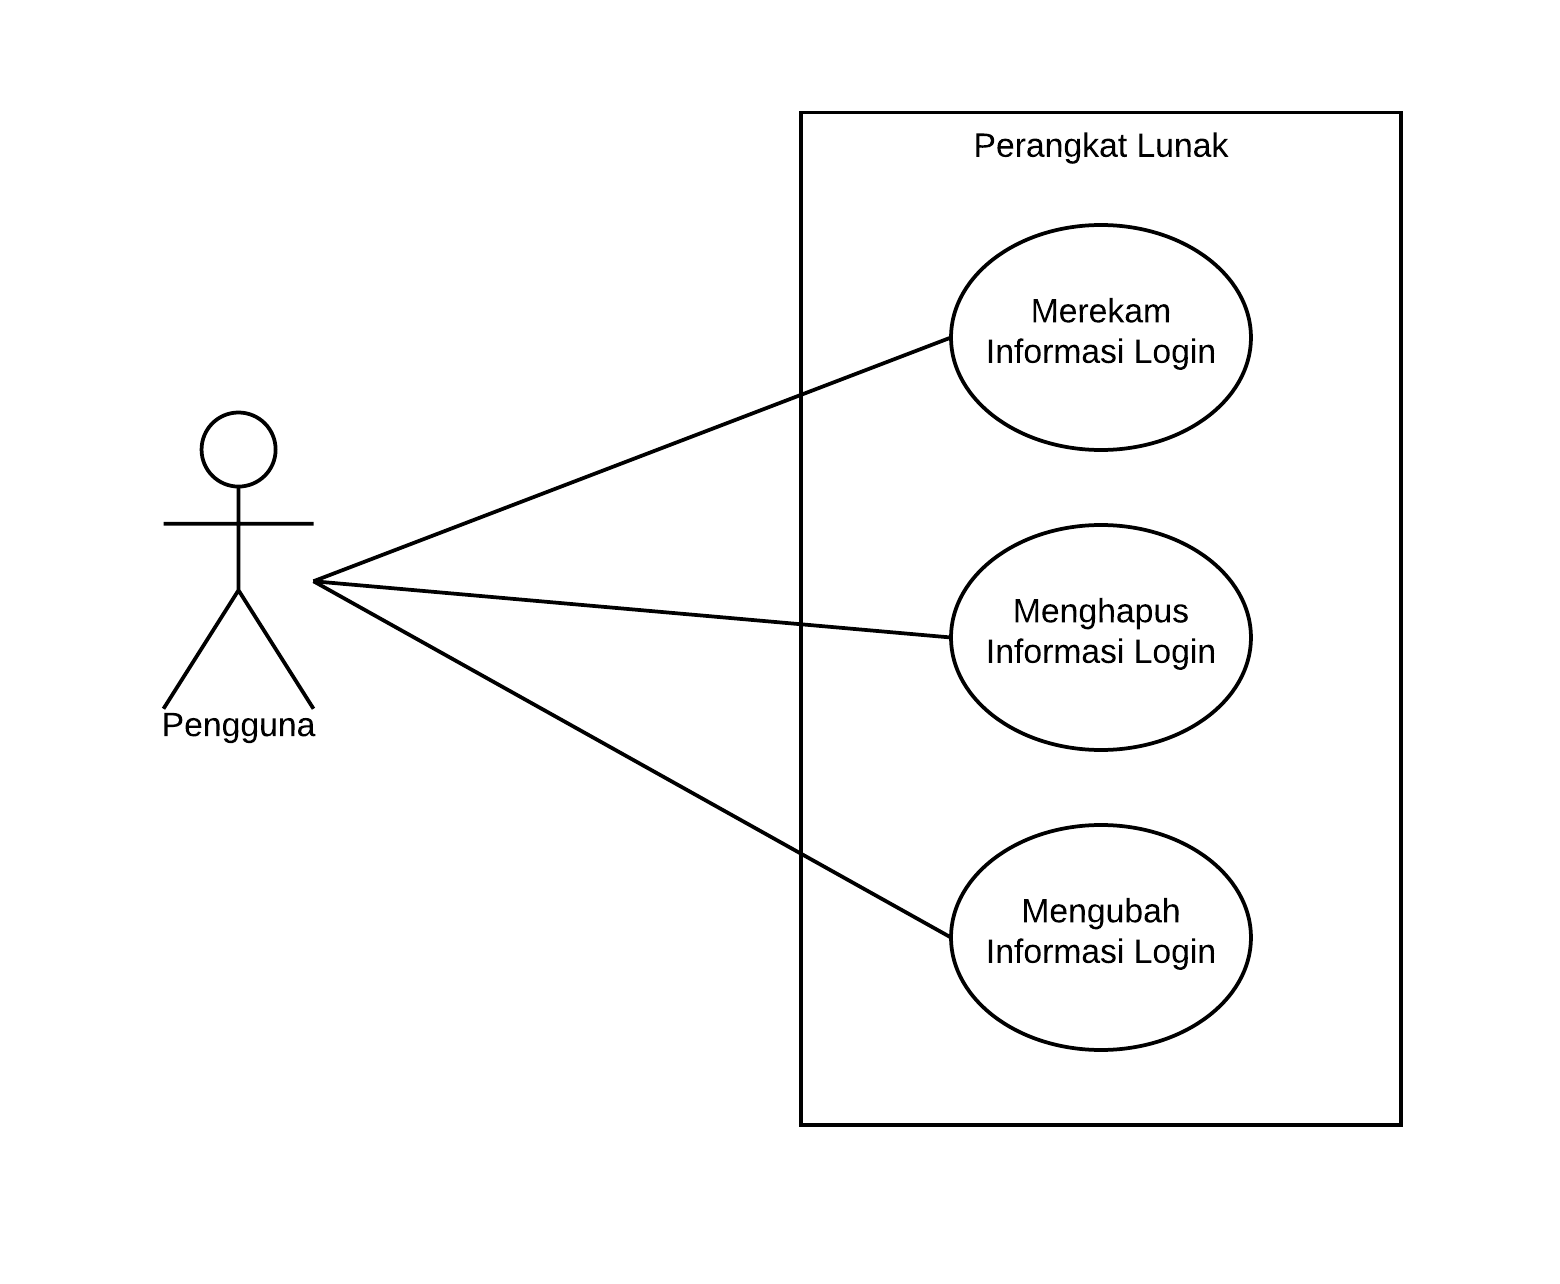
\includegraphics[scale=0.77]{usecase.png}
            \caption[Diagram \textit{use case} untuk perangkat lunak yang dibangun.]{Diagram \textit{use case} untuk perangkat lunak yang dibangun.}
            \label{fig:usecase}
        \end{figure}

        \textbf{Skenario merekam informasi login}
        
        Nama: Merekam informasi login\\
        Aktor: Pengguna\\
        Kondisi awal: Perangkat lunak mendeteksi adanya \textit{captive portal}.\\
        Deskripsi: Pengguna menyimpan informasi login.\\
        Kondisi Akhir: Informasi login tersimpan di dalam perangkat lunak.\\\\
        Skenario:
        \begin{enumerate}
            \item{Pengguna memasukkan informasi login ke dalam form HTML.}
            \item{Sistem menyimpan informasi login yang dimasukkan oleh pengguna.}
        \end{enumerate}

        \textbf{Skenario menghapus informasi login}
        
        Nama: Menghapus informasi login\\
        Aktor: Pengguna\\
        Kondisi awal: Perangkat lunak sudah dijalankan.\\
        Deskripsi: Pengguna menghapus informasi login.\\
        Kondisi Akhir: Informasi login dihapus dari perangkat lunak.\\\\
        Skenario:
        \begin{enumerate}
            \item{Pengguna memilih untuk menghapus informasi login.}
            \item{Sistem menghapus informasi login.}
        \end{enumerate}

        \textbf{Skenario mengubah informasi login}
        
        Nama: Mengubah informasi login\\
        Aktor: Pengguna\\
        Kondisi awal: Perangkat lunak sudah dijalankan.\\
        Deskripsi: Pengguna mengubah informasi login.\\
        Kondisi Akhir: Informasi login diubah dari perangkat lunak.\\\\
        Skenario:
        \begin{enumerate}
            \item{Pengguna memilih untuk mengubah informasi login.}
            \item{Sistem menampilkan form ubah informasi login.}
            \item{Pengguna memasukkan informasi login baru.}
            \item{Sistem menghapus informasi login lama dan menyimpan informasi login baru.}
        \end{enumerate}
        
        \textbf{Skenario memicu login otomatis}
        
        Nama: Memicu login otomatis\\
        Aktor: WiFi\\
        Kondisi awal: Perangkat lunak sudah dijalankan.\\
        Deskripsi: Sistem memicu login otomatis berdasarkan perubahan status WiFi.\\
        Kondisi Akhir: klien terotentikasi pada \textit{captive portal}.\\\\
        Skenario:
        \begin{enumerate}
            \item{Sistem mendeteksi adanya koneksi WiFi yang terjadi.}
            \item{Sistem mendeteksi adanya \textit{captive portal}.}
            \item{Sistem mendeteksi adanya informasi login untuk \textit{captive portal} tersebut.}
            \item{Sistem mengirimkan informasi login kepada \textit{captive portal}.}
            \item{Sistem mendeteksi koneksi dengan internet dan klien sudah terotentikasi pada \textit{captive portal} tersebut.}
        \end{enumerate}
        
        Diagram Kelas:
        
        \begin{figure}[h]
            \centering
            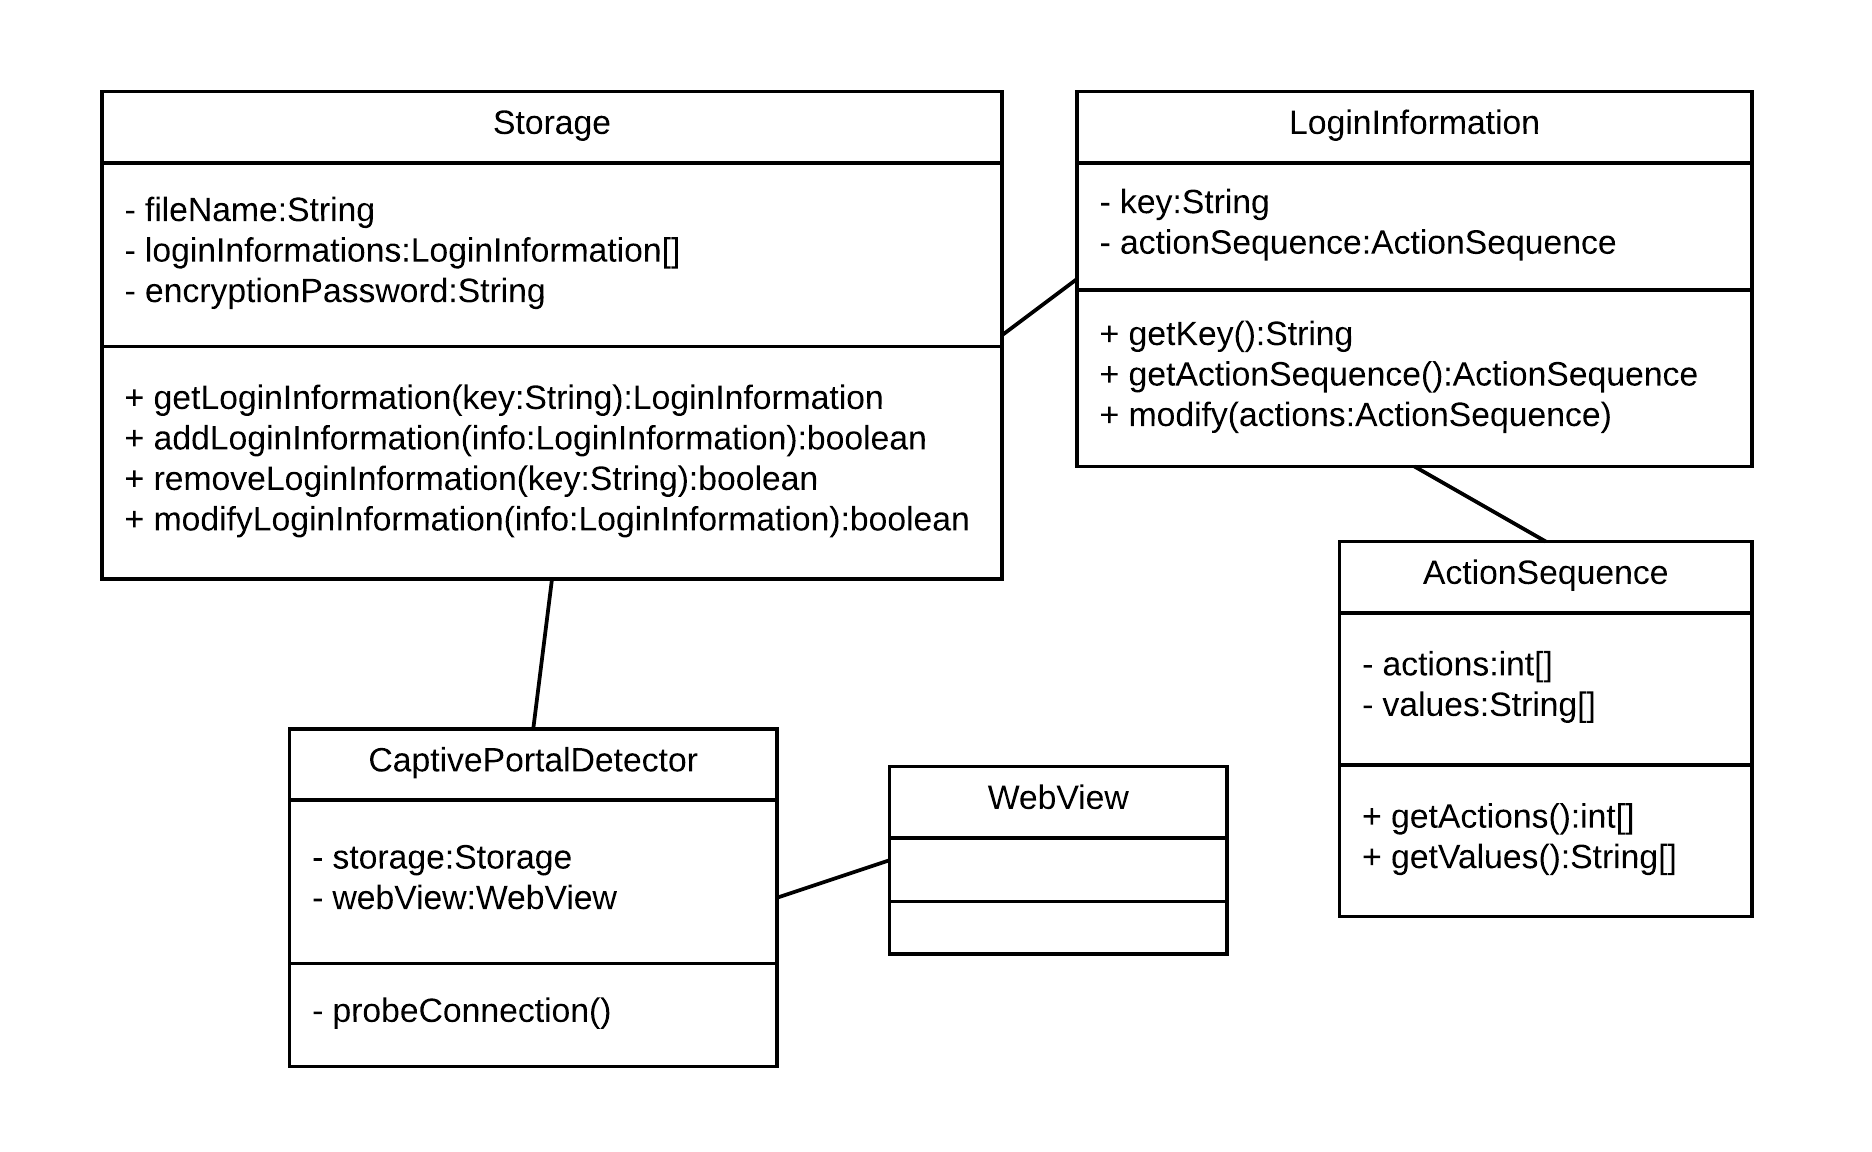
\includegraphics[scale=0.85]{classdiagram.png}
            \caption[Diagram kelas untuk perangkat lunak yang dibangun.]{Diagram kelas untuk perangkat lunak yang dibangun.}
            \label{fig:diagramkelas}
        \end{figure}
        
        Kelas-kelas yang dibutuhkan pada perangkat lunak ini adalah:
        
        \begin{itemize}
            \item{CaptivePortalDetector\\Kelas ini digunakan untuk mendeteksi keberadaan \textit{captive portal}. Jika captive portal terdeteksi, maka informasi login yang tersimpan dalam Storage digunakan. Jika tidak terdapat informasi login dalam Storage, maka direkam informasi login baru.}
            \item{Storage\\Kelas ini digunakan untuk menyimpan seluruh informasi login dalam bentuk file teks yang sudah terenkripsi.}
            \item{LoginInformation\\Kelas ini digunakan untuk menyimpan informasi login dalam bentuk key atau fingerprint, serta ActionSequence}
            \item{ActionSequence\\Kelas ini digunakan untuk menyimpan langkah-langkah login dalam bentuk urutan aksi dan nilai-nilai yang berkaitan dengan aksi tersebut.}
        \end{itemize}

		\item Merancang perangkat lunak login otomatis ini\\
		{\bf status :} Ada sejak rencana kerja skripsi.\\
		{\bf hasil :} Dilaksanakan pada Skripsi 2.

		\item  Melakukan pengujian terhadap perangkat lunak untuk menghasilkan perbaikan teradap perangkat
lunak tersebut.\\
		{\bf status :} Ada sejak rencana kerja skripsi. \\
		{\bf hasil :} Dilaksanakan pada Skripsi 2.

		\item Membuat kesimpulan dari hasil penelitian dan saran untuk penelitian selanjutnya.\\
		{\bf status :} Ada sejak rencana kerja skripsi.\\
		{\bf hasil :} Dilaksanakan pada Skripsi 2.

		\item Melakukan pengujian (dan eksperimen) yang melibatkan responden untuk menilai hasil simulasi secara kualitatif\\
		{\bf status :} Ada sejak rencana kerja skripsi.\\
		{\bf hasil :} Dilaksanakan pada Skripsi 2.

		\item Menulis dokumen skripsi.\\
		{\bf status :} Ada sejak rencana kerja skripsi.\\
		{\bf hasil :} Sudah dikerjakan sampai dengan bab 3 (Analisis).

	\end{enumerate}

\pagebreak

\section{Pencapaian Rencana Kerja\footnote{Terdapat kesalahan pada dokumen rencana kerja terdahulu di mana terdapat 8 poin rencana kerja, sementara hanya tertera 7 poin pada tabel rencana kerja. Poin-poin rencana kerja yang benar adalah yang ada pada dokumen ini.}}

Persentase penyelesaian skripsi sampai dengan dokumen ini dibuat dapat dilihat pada tabel berikut :

\begin{center}
  \begin{tabular}{ | c | c | c | c | l | c |}
    \hline
    1*  & 2*(\%) & 3*(\%) & 4*(\%) &5* &6*(\%)\\ \hline \hline
    1   & 5  & 5  &  &  & 5 \\ \hline
    2   & 10 & 10  &   &  & 10 \\ \hline
    3   & 15  & 10  & 5 & {\footnotesize kaji ulang singkat kebutuhan pada S2}  & 10  \\ \hline
    4   & 10  &  & 10 &  & \\ \hline
    5   & 15  &   & 15 & & \\ \hline
    6   & 10 &   & 10  & & \\ \hline
    7   & 5 &   & 5  & & \\ \hline
    8   & 30  & 15  & 15 & {\footnotesize sebagian bab 1 dan 2, serta bagian awal analisis di S1} & 15 \\ \hline
    Total  & 100  & 40  & 60 &  & 40\\ \hline
                          \end{tabular}
\end{center}

Keterangan (*)\\
1 : Bagian pengerjaan Skripsi (nomor disesuaikan dengan detail pengerjaan di bagian 5)\\
2 : Persentase total \\
3 : Persentase yang akan diselesaikan di Skripsi 1 \\
4 : Persentase yang akan diselesaikan di Skripsi 2 \\
5 : Penjelasan singkat apa yang dilakukan di S1 (Skripsi 1) atau S2 (skripsi 2)\\
6 : Persentase yang sidah diselesaikan sampai saat ini

%\section{Kendala yang dihadapi}
%%TULISKAN BAGIAN INI JIKA DOKUMEN ANDA TIPE A ATAU C
%Kendala - kendala yang dihadapi selama mengerjakan skripsi :
%\begin{itemize}
	%\item Terlalu banyak melakukan prokratinasi
	%\item Terlalu banyak godaan berupa hiburan (game, film, dll)
	%\item Skripsi diambil bersamaan dengan kuliah ASD karena selama 5 semester pertama kuliah tersebut sangat dihindari dan tidak diambil, dan selama 4 semester terakhir kuliah tersebut selalu mendapat nilai E
	%\item Mengalami kesulitan pada saat sudah mulai membuat program komputer karena selama ini selalu dibantu teman
%\end{itemize}

\vspace{1cm}
\centering Bandung, \tanggal\\
\vspace{2cm} \nama \\ 
\vspace{1cm}

Menyetujui, \\
\ifdefstring{\jumpemb}{2}{
\vspace{1.5cm}
\begin{centering} Menyetujui,\\ \end{centering} \vspace{0.75cm}
\begin{minipage}[b]{0.45\linewidth}
% \centering Bandung, \makebox[0.5cm]{\hrulefill}/\makebox[0.5cm]{\hrulefill}/2013 \\
\vspace{2cm} Nama: \pembA \\ Pembimbing Utama
\end{minipage} \hspace{0.5cm}
\begin{minipage}[b]{0.45\linewidth}
% \centering Bandung, \makebox[0.5cm]{\hrulefill}/\makebox[0.5cm]{\hrulefill}/2013\\
\vspace{2cm} Nama: \pemB \\ Pembimbing Pendamping
\end{minipage}
\vspace{0.5cm}
}{
% \centering Bandung, \makebox[0.5cm]{\hrulefill}/\makebox[0.5cm]{\hrulefill}/2013\\
\vspace{2cm} Nama: \pembA \\ Pembimbing Tunggal
}

\end{document}

